\section{Overview}
In this section, we present a high level overview of EDP and highlight its
benefits in understanding energy and time trade-offs that exist in a contrived
example. Next, we delve into details of the hardware parameters studied in this
work.

%\subsection{Energy Delay Product (EDP)}
%\label{sec:overview}
%%\paragraph{What does it mean to optimize energy consumption?}
%\begin{figure}
%	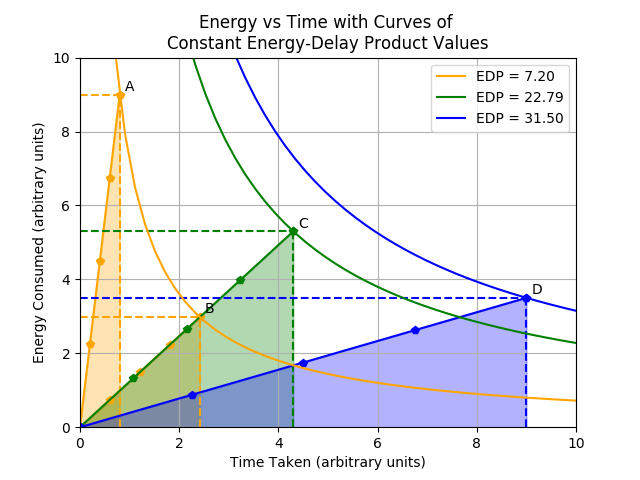
\includegraphics[width=7.7cm]{figures/EDP_AbstractPlot.png}
%	\caption{Generic EDP plot}
%	\label{fig:edp}
%\end{figure}
%% YA
%
In datacenters, time and energy is money, and both are required to get a piece
of computational work done. The relationship between them can give us insight
into the interactions between the application, the underlying OS, and the
hardware. We define a single metric that embeds information about both relevant
computational costs: energy and time. EDP captures this relation by simply
multiplying how much time a computation takes with how much energy is consumed.
For any fixed workload in a datacenter, it is always preferable to minimize EDP
as it results in using less time to get said work done along with less energy.
Using EDP plots, we can determine if a method is strictly better than another
in terms of both time and energy or if the trade-off between the two is more
subtle.

EDPs can also be useful for capturing behaviors in different methods  getting
the same piece of work done.
It is easy to measure how long a computation takes and the total amount of
energy a computer uses to run a application can be measured on its main power
line.
%% EDP has units of Joule Seconds (J s)
%
The Energy Delay Product (EDP) is a single numeric value that captures this
relationship between the time and energy required to do some work: it is
computed as the product of all Joules measured and the total time taken to do
said work. This value can also be used as a means for comparing different
methods for getting the same piece of work done.
%
%
%%6As such, we use EDP as the main plots to present our efficiency results.
%%EDP is a general measure that accounts for the value of both energy and time. 
%%Moreover, it is also useful to compare the efficiencies of these two methods
with respect to a workload specific measure such as bytes processed per Joule
or some operation per Joule. When considering latency sensitive work, it might
also be useful to consider a more complex scenario such as the distribution of
latency's with respect to the energy consumed. With this in mind, we also seek
to derive some workload specific efficiency measures catered to each
application.
%
%%% YA
%%As the old adage goes, "time is money".  Similarly, "energy is money", as it
takes both time and energy to get some work done.
%%To capture this relationship and compare various options for getting some
particular work done, it is useful to consider Energy Delay Product (EDP): the
product of the energy - all Joules measured to do the work - and delay - total
time to do the work.
%%This product is referred to as the Energy Delay Product (EDP) and can be
expressed as $Joules \times Seconds$.
%%Where Energy is the sum of all the Joules measured to do the work and Delay
is the total time to do the work.
%%While EDP is a single number, and useful for comparing methods,  plotting the
energy consumed over the life time of methods reveals more insight between how
methods compare.
%
%
%Figure~\ref{fig:edp}, is a generic EDP plot of three different methods for
doing a particular task. If energy is consumed at a constant rate, then a
straight line captures the method's behavior and the area under the curve is
its EDP.
%%While one is rarely disappointed if it takes both less time and less energy
to do some work, more often than not, the tradeoff in the time and energy, that
given methods for doing the work has or the utility that time or energy has to
you results in more subtly comparisons.
%%Evaluating EDP plots helps quantify the relationships in differing methods.  
%%An EDP plot shows the running sum of energy consumed as a particular method
proceeds in doing the given work.
%%The area under the curve of a method's temporal energy consumption is its EDP.
%%Figure~\ref{fig:edp} also shows the behavior in which energy is consumed at a
constant rate, the straight
%%If energy is consumed at a constant rate, as is the case for the four methods
in Figure~\ref{fig:edp}, a straight line captures the methods behaviour and the
area is simply the total delay multiplied by the total energy.
%While a particular value for EDP might be constant for two methods, their
respective time-to-energy trade-offs might be quite different.
%The colored EDP lines illustrate this relationship:
%while methods A and B have the same EDP, there is a clear difference in their
time and energy trade-offs. When considering methods B and C, B has a smaller
EDP value and is clearly better with respect to both time and energy.
%The rate of energy consumption is reflected by the slope of the EDP plots.
%%On the other hand, if one cares about the rate of power consumption between
two methods, it is reflected in the slope of the EDP plots.
%Method D has the lowest rate of energy consumption but takes more than 4 times
as long as method B.
%While B is also better than D in terms of total energy consumed, its rate of
consumption is much higher, and this could be an important factor in some
scenarios where pricing is taken into account.
%
%\subsection{Methdology}
%\label{sec:setup}

%\begin{wrapfigure}{r}{.6\columnwidth}
%%\vspace{-0.24in}
%\begin{center}
  %%\hspace{-.22in}
%  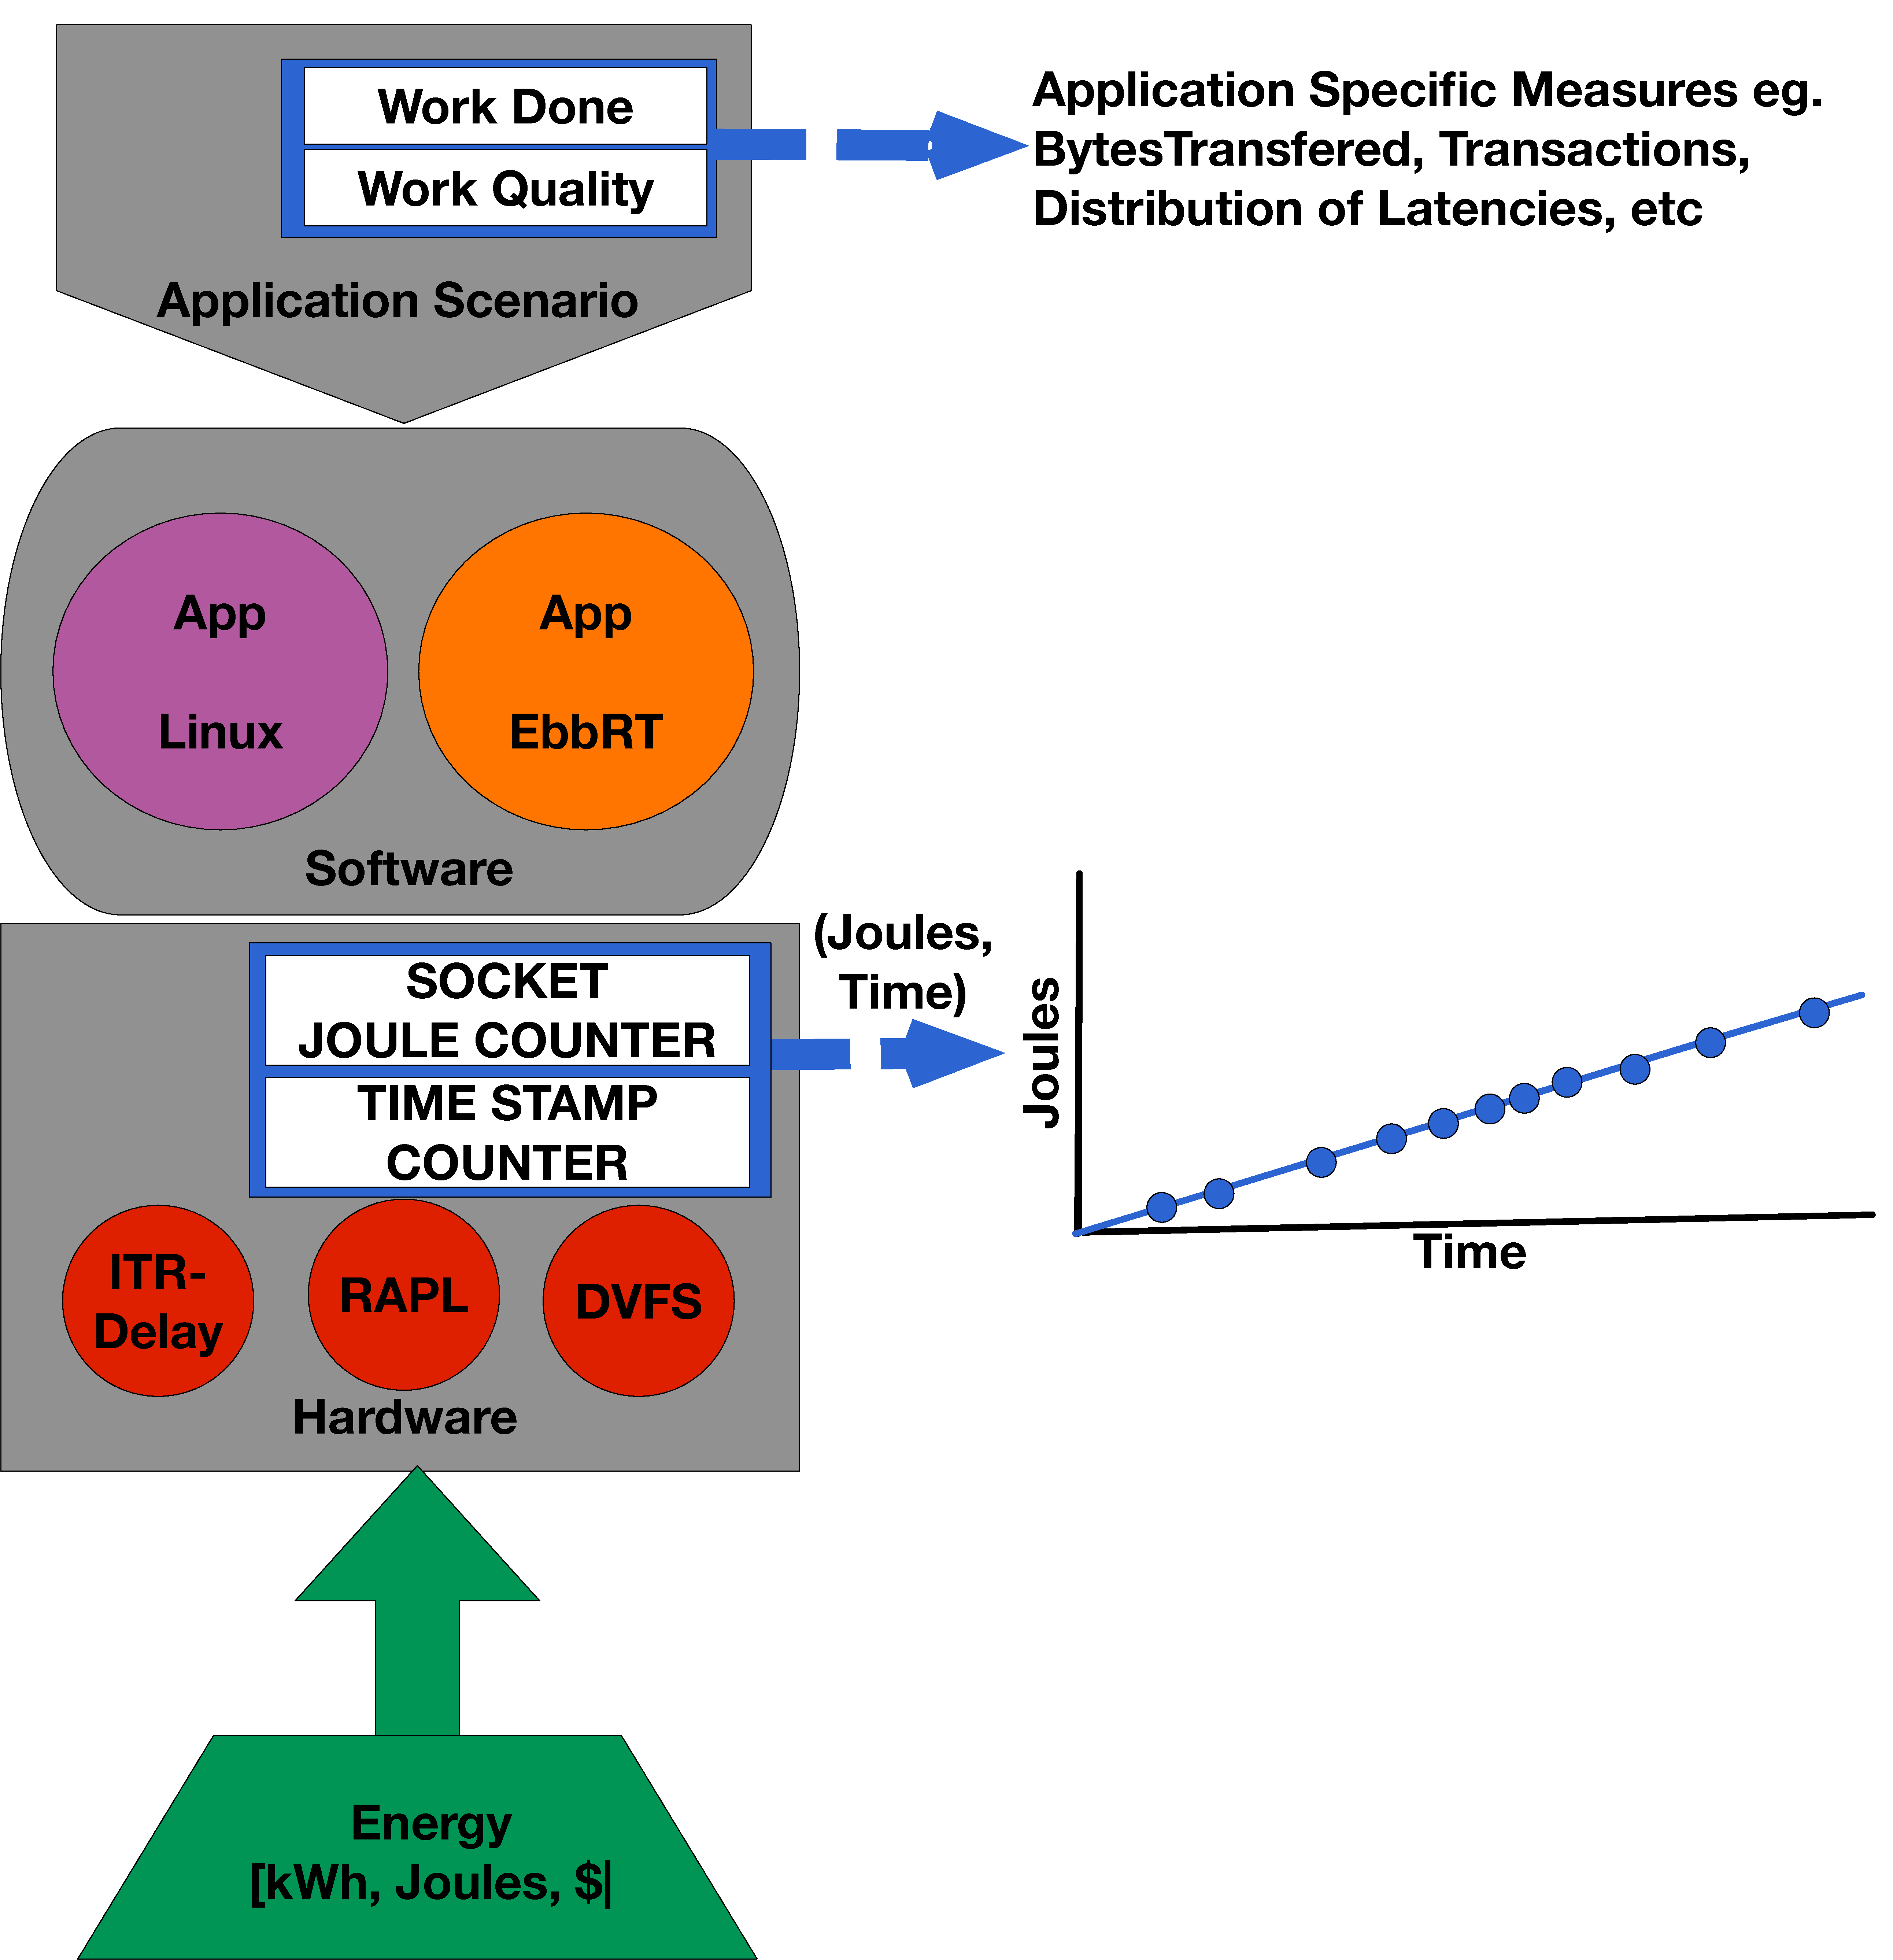
\includegraphics[width=.7\columnwidth]{figures/setup.pdf}
%%\vspace{-.24in}
%\caption{Setup}
	%\label{fig:setup}
%%	\vspace{-.2in}
%	\end{center}	
%\end{wrapfigure}

%Figure~\ref{fig:setup}, illustrates our general setup for studying energy
optimization.   Abstractly the hardware and software that composes a server
configuration consumes energy in the form of electricity measured in Joules to
complete some application specific work.

%Our specific hardware and networking infrastructure is described
in~\ref{sec:hw}. We consider the of tuning three settings; 1) NIC ITR-Delay, 2)
Processor Dynamic Voltage Frequency Scaling, and 3) Processor Running Power
Limits.  We discuss these in more detail in~\ref{sec:knobs}.  We also use
features of the hardware to measure the running number of Joules consumed
within the processor package whenever a NIC interrupt occurs. Each value is
timestamped using the processors timestamp counter. In this way we obtain EDP
data.  This measurement strategy is discussed  in more detail
in~\ref{sec:measures}.

%We examine four application scenarios (~\ref{sec:apps}), driving the system
with  application specific workloads.  For each workload we define a measure to
tune and compare the efficiency of the system configurations.

%While the hardware platform is fixed, beyond the parameters we tune, the
software configuration is the main variable we are studying.  Our goal is to
reveal the impact of two software stacks on power tuning power; 1) Linux
configured to run the single application service and 2) an application specific
bare-metal ebbrtlibrary OS built for the service.  Section~\ref{sec:stacks}
describes these two software stacks, how we configure them and our energy
tuning methodology.

%Our data reveals both the self-relative impact of tuning the hardware
parameters considered for each software stack and how they compare against each
other. The next subsection (~\ref{sec:findingsum}) summarizes the core
findings.

%\subsection{Summary of Core Findings}
%\label{sec:findingsum}
%\begin{table*}[t]
\begin{center}
%\begin{adjustbox}{angle=90}
\begin{tabular}{|l|cc|cc|cc||cc|cc} \hline
\multirow{2}{*}{Workload} & \multicolumn{6}{c|}{Linux} & \multirow{2}{*}{}\\ 
& \multicolumn{2}{c}{Default} & \multicolumn{2}{c}{Tuned: DVFS} & \multicolumn{2}{c|}{Tuned: DVFS + ITR} \\
\hline

 & EDP (Js)& TPUT & EDP (Js) & TPUT & EDP (Js) & TPUT \\  
 \hline

Netpipe: 64 B & $0.486 \pm 0.005$ & $0.150 \pm 0.001$ & $0.349 \pm 0.003$ & $0.185 \pm 0.001$ & $0.240 \pm 0.008$ & $0.226 \pm 0.003$ \\ \hline
Netpipe: 8 KB & $14.653 \pm 0.206$ & $3.195 \pm 0.023$ & $13.388 \pm 3.604$ & $3.548 \pm 1.043$ & $1.033 \pm 0.007$ & $14.752 \pm 0.046$ \\ \hline
Netpipe: 64 KB & $28.311 \pm 6.267$ & $19.940 \pm 1.971$ & $26.498 \pm 11.608$ & $21.567 \pm 5.069$ & $10.034 \pm 0.356$ & $36.154 \pm 0.611$ \\ \hline
Netpipe: 512 KB & $308.329 \pm 1.496$ & $50.855 \pm 0.056$ & $274.978 \pm 0.938$ & $50.485 \pm 0.064$ & $263.681 \pm 0.426$ & $52.422 \pm 0.026$ \\ \hline
\hline
\end{tabular}
%\end{adjustbox}
\end{center}
\label{tab:netpipe_linux}
\end{table*}

%% netpipe ebbrt
\begin{table*}[t]
\begin{center}
%\begin{adjustbox}{angle=90}
\begin{tabular}{|l|cc|cc|cc||cc|cc||c|} \hline

\multirow{2}{*}{Workload} & \multicolumn{4}{c|}{ebbrt} & \multirow{2}{*}{Net Savings}\\ 
& \multicolumn{2}{c}{BaseLine} & \multicolumn{2}{c|}{Tuned} &\\
\hline
 & EDP (Js)& $TPUT$ & EDP (Js) & $TPUT$ & \\  \hline

Netpipe: 64 B & $0.246 \pm 0.003$ & $0.196 \pm 0.001$ & $0.140 \pm 0.005$ & $0.287 \pm 0.002$ \\ \hline
Netpipe: 8 KB & $0.597 \pm 0.022$ & $17.625 \pm 0.280$ & $0.511 \pm 0.004$ & $18.961 \pm 0.063$ \\ \hline
Netpipe: 64 KB & $6.248 \pm 0.013$ & $42.264 \pm 0.034$ & $4.691 \pm 0.009$ & $45.761 \pm 0.026$ \\ \hline
Netpipe: 512 KB & $224.042 \pm 0.100$ & $54.385 \pm 0.007$ & $206.815 \pm 0.087$ & $54.769 \pm 0.013$ \\ \hline

\hline \hline
\end{tabular}
%\end{adjustbox}
\end{center}
\label{tab:netpipe_ebbrt}
\end{table*}

%% nodeJS linux
\begin{table*}[t]
\begin{center}
%\begin{adjustbox}{angle=90}
\begin{tabular}{|l||cc|cc||cc||c|} \hline
\multirow{2}{*}{Workload} & \multicolumn{6}{c|}{Linux} & \multirow{2}{*}{Net Savings}\\ 
& \multicolumn{2}{c}{Default} & \multicolumn{2}{c}{Tuned: DVFS} & \multicolumn{2}{c|}{Tuned: DVFS + ITR} &\\
\hline

 & EDP (Js)& RPS & EDP (Js) & RPS & EDP (Js) & RPS & \\  \hline

NodeJS: & $14701.049 \pm 124.418$ & $11.932 \pm 0.070$ & $12864.951 \pm 122.798$ & $11.119 \pm 0.086$ & $14766.383 \pm 162.696$ & $13.126 \pm 0.059$ \\ \hline

\hline \hline
\end{tabular}
%\end{adjustbox}
\end{center}
\end{table*}

%%nodeJS ebbrt
\begin{table*}[t]
\begin{center}
%\begin{adjustbox}{angle=90}
\begin{tabular}{|l|cc|cc|cc||cc|cc||c|} \hline

\multirow{2}{*}{Workload} & \multicolumn{4}{c|}{ebbrt} & \multirow{2}{*}{Net Savings}\\ 
& \multicolumn{2}{c}{BaseLine} & \multicolumn{2}{c|}{Tuned} &\\
\hline
 & EDP (Js)& RPS & EDP (Js) & RPS & \\  \hline

NodeJS: & $14200.412 \pm 73.321$ & $16.919 \pm 0.601$ & $12634.927 \pm 7.875$ & $16.576 \pm 0.165$ \\ \hline

\hline \hline
\end{tabular}
%\end{adjustbox}
\end{center}
\end{table*}


%% memcached linux
\begin{table*}[t]
\begin{center}
%\begin{adjustbox}{angle=90}
\begin{tabular}{|l||cc|cc||cc||c|} \hline
\multirow{2}{*}{Workload} & \multicolumn{6}{c|}{Linux} & \multirow{2}{*}{Net Savings}\\ 
& \multicolumn{2}{c}{Default} & \multicolumn{2}{c}{Tuned: DVFS} & \multicolumn{2}{c|}{Tuned: DVFS + ITR} &\\
\hline

 & EDP (Js)& RPS & EDP (Js) & RPS & EDP (Js) & RPS & \\  \hline

Memcached: 200000 rps & $29824.673 \pm 7.121$ & $1987.914 \pm 0.672$ & $37880.483 \pm 36.185$ & $2524.524 \pm 2.412$ & $23855.600 \pm 35.121$ & $1590.373 \pm 2.341$ \\ \hline
Memcached: 400000 rps & $43064.080 \pm 121.605$ & $2869.982 \pm 8.104$ & $43732.463 \pm 39.602$ & $2914.526 \pm 2.639$ & $26362.600 \pm 45.517$ & $1757.507 \pm 3.034$ \\ \hline
Memcached: 600000 rps & $58008.190 \pm 69.067$ & $3865.924 \pm 4.603$ & $48437.701 \pm 7.348$ & $3228.104 \pm 0.490$ & $37388.963 \pm 4509.272$ & $2492.597 \pm 300.618$ \\ \hline


\hline \hline
\end{tabular}
%\end{adjustbox}
\end{center}
\end{table*}

%%memcached ebbrt
\begin{table*}[t]
\begin{center}
%\begin{adjustbox}{angle=90}
\begin{tabular}{|l|cc|cc|cc||cc|cc||c|} \hline

\multirow{2}{*}{Workload} & \multicolumn{4}{c|}{ebbrt} & \multirow{2}{*}{Net Savings}\\ 
& \multicolumn{2}{c}{BaseLine} & \multicolumn{2}{c|}{Tuned} &\\
\hline
 & EDP (Js)& RPS & EDP (Js) & RPS & \\  \hline

Memcached: 200000 rps & $21185.300 \pm 9.297$ & $1412.353 \pm 0.620$ & $21109.500 \pm 33.851$ & $1407.300 \pm 2.257$ \\ \hline
Memcached: 400000 rps & $22205.150 \pm 27.923$ & $1480.343 \pm 1.862$ & $22132.200 \pm 65.861$ & $1475.480 \pm 4.391$ \\ \hline
Memcached: 600000 rps & $26413.000 \pm 309.029$ & $1760.867 \pm 20.602$ & $23201.900 \pm 16.807$ & $1546.793 \pm 1.120$ \\ \hline

\hline \hline
\end{tabular}
%\end{adjustbox}
\end{center}
\end{table*}


%It might be useful to have an overview table of the results and summary of the
causal analysis here.

%Normalize results to Linux where possible

%Extract and quantify efficiency at the instruction and energy level.

% In contrast to Linux, EbbRT uses a re-implemented version of memcached
written to EbbRT interfaces. It is a multicore application that supports the
standard memcached binary protocol. To alleviate lock contention, a RCU
hashtable is used to store key-value pairs. EbbRT's implementation does lack
some additional features such as authentication and other commands but it is
functional enough to support the benchmark tool.
%We run memcached-1.5.6 on top of a Ubuntu LTS 18.0.4 installation with Linux
4.15.1, the other nodes either run Ubuntu LTS 18.0.4 with a mix of Linux 4.15.1
and 5.0.0 or Red Hat Enterprise Linux 7.7 with Linux 3.10.0.

%The same server node is also used to boot into baremetal EbbRT. It contains a
16 core Intel(R) Xeon(R) CPU E5-2690 @ 2.90GHz, with 125 GB of RAM and a Intel
Corporation 82599ES 10-Gigabit SFI/SFP+ NIC. In contrast to Linux, EbbRT uses a
re-implemented version of memcached written to EbbRT interfaces. It is a
multicore application that supports the standard memcached binary protocol. To
alleviate lock contention, a RCU hashtable is used to store key-value pairs.
EbbRT's implementation does lack some additional features such as
authentication and other commands but it is functional enough to support the
benchmark tool.



\section{Network Device Drivers}
\begin{figure}
  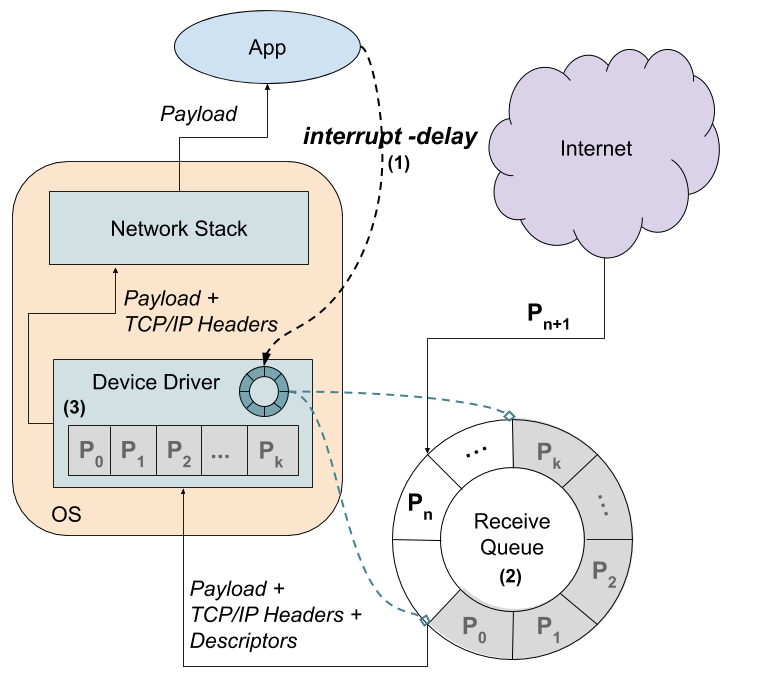
\includegraphics[width=7.7cm]{itr_figure.png}
\caption{As interrupt delay (1) is increased, the receive queue (2) buffers
more incoming packets as the NIC cannot fire new interrupts until the delay
value has been reached. Once the interrupt is fired, Linux's NAPI polling
mechanism kicks in and starts pulling in new packets (3) to be processed until
it either reaches its current work budget (calculated using existing jiffies)
or until there is no more data to be processed.}
  \label{fig:itr_figure}
\end{figure}

\subsection{Hardware Tuning Parameters}
Below, we discuss the three hardware parameters that are tuned statically in
this work:
\label{sec:knobs}
\begin{itemize}
\item \textbf{interrupt-delay}: Most modern NICs have a hardware feature to
control per receive interrupt rates.
The Intel 82599 datasheet~\cite{82599} defines a time-based interrupt
throttling mechanism which controls the time delay between packet reception and
the firing of an interrupt on the receiving core.
Its value can be set from a range between \texttt{0} and \texttt{1024}
$\micro$s in increments of \texttt{2} $\micro$s.
Figure~\ref{fig:itr_figure} illustrates the interaction of interrupt delay
values with the rest of systems software.
The effect of setting a higher interrupt delay results in potential buffering
of receive packets, thereby increasing packet processing efficiency at a
potential cost to response time.

Linux's network device driver uses a dynamic algorithm that seeks to tune the
interrupt delay value such that it better reflects the current workload.
It achieves this by using data received from the previous interrupt about
packet counts and bytes per packet.
These values are then used to classify the current state of the workload (ex:
latency driven vs. bulk compute) and tune the interrupt delay accordingly based
off pre-computed theoretical maximum wire speeds.
%received from the last interrupt and classifies them broadly into a set of
ranges that are pre-computed based off theoretical maximum wire speeds.
%This delay tuning is applied upon the next interrupt occurrence.
It is possible to disable this dynamic algorithm through the flip of a bit
inside the device driver. After flipping this bit, \textit{ethtool} can then be
used to set new interrupt delay values to statically fire at a fixed rate.
In our experiments, we take advantage of this ability by setting interrupt
delay values statically for different applications.
%device driver [REF] updates the interrupt delay value dynamically after every
packet receive to a value based on the current traffic pattern. This value can
also be fixed to a static value which results in interrupts being fired every X
microseconds where X is a configurable value.


%To demonstrate its behavior, we instrumented a simple logging tool into the
IXGBE device driver.
%Figure~\ref{fig:itr_delays} shows a small snapshot of its values while running
a Memcached workload.
%Each marker represents a new \textit{ITR-Delay} value.
%In its current implementation, it can only seek values between the range of 2
to 126 microseconds.
%The reason for this is that it was never designed towards a use case of
aggressively delaying packet receive interrupts to take advantage of energy
proportionality under stringent SLAs, which can potentially result in setting
\textit{ITR-Delay} values in the hundreds of microseconds.

%It is also possible to disable this dynamic algorithm through the flip of a
bit inside the device driver.
%This requires a rebuild of the driver module as it was not a configurable
parameter.
%After flipping this bit, we can use Linux's \textit{ethtool} to set new
interrupt delay values statically to fire every X microseconds, where X is a
configurable value.


\item \textbf{RAPL}: Running Average Power Limit (RAPL)~\cite{intel_rapl} is a
power limiting feature on Intel processors.
In our experiments, we use the RAPL model segment registers (MSR) registers to
set explicit power limits up to a default max of \texttt{135} Watts (\watt) in
a single package on the processor. The processor used in our experiments
contain two packages. When applying power limits, care must be taken to ensure
there is a minimum RAPL value such that an application's continued execution
can be sustained in this limited power budget.
%Applications often depend on hardware components that in turn rely on a
minimum power supply to continue running.
%Hence, when considering energy efficient compute, calculating minimum RAPL
values that would sustain the execution of a particular workload becomes
important.
From some initial experiments, we found that our class of applications
continued to execute correctly at a minimum RAPL limiting of around \texttt{55}
\watt. RAPL also provides the MSR\_PKG\_ENERGY\_STATUS register which allows
software to query the energy usage (Joules) of a specific package with a
minimum sample time of 1 milliseconds.
This is the main method with which our per-application energy consumption
results are gathered.

\item \textbf{DVFS}: Intel power states (p-states) is another energy saving
feature on Intel processors.
It allows users to set specific p-states for individual cores.
A p-state is a combination of the clock frequency and voltage that a core is
operating on. Typically,  p-states are set dynamically according to current
processor load by a policy governor in Linux called Dynamic Voltage Frequency
Scaling (DVFS). DVFS can be disabled, thereby enabling setting static p-state
values by writing to the IA32\_PERF\_CTL register~\cite{intel_msr}.
%A p-state is the combination of a core's clock frequency and its voltage at
some ratio, however, it is also unclear how it translates to real processor
frequency.
%Normally, p-states are set dynamically according to current processor load by
a policy governor in Linux called Dynamic Voltage Frequency Scaling (DVFS).
%In addition, DVFS can also be disabled which enables a user to set specific
p-state values by writing to the IA32\_PERF\_CTL register~\cite{intel_msr}.
From reading MSR\_PERF\_STATUS register~\cite{intel_msr}, we found the range of
DVFS values that a default Linux sets its processor into starts at a minimum
value of \texttt{0xC00} and up to a maximum of \texttt{0x1D00}. We use this
range in our study to tune processor p-states as another hardware knob.
\end{itemize}

\subsection{Per-interrupt Log Collection}
\label{sec:log_collect}
In order to better understand the interactions of interrupt-delay, DVFS, and
RAPL with a server that is under some load, we instrument \textit{fine-grained
per-interrupt} log collection in both Linux and library OS's network device
driver.
We collect the following information for every interrupt fired: received and
transmitted bytes, received and transmitted descriptors, and the current
timestamp (via \texttt{rdtsc} instruction).
In addition, we instrument per-core performance monitoring counters (PMCs) to
collect a set of hardware statistics after every millisecond of elapsed time:
instructions, cycles, reference cycles, last-level cache misses, and energy
used (using the MSR\_PKG\_ENERGY\_STATUS register).
This set of statistics helps us to both take a detailed look at the per-core
behavior and acquire a global perspective on overall resource usage when
hardware is tuned in different ways.
%While this data provides a breadth of directions to reason about the results
below, we discovered that it can be helpful to focus on subsets of data points
for different workloads.
We ensure that the logging mechanism adds minimal overhead to application
performance by using non-temporal store instructions to store the collected
statistics into an in-memory array.
%We found that using non-temporal store instructions had more of an impact on
the performance of EbbRT versus that of Linux.
%We believe that this could be due to the fact that EbbRT was built to be an
efficient library OS and hence its performance is more observably affected by
additional logging.
%\subsubsection{Measurements}
%\label{sec:measures}
%\begin{itemize}
%       \item Throughput and Latency: Throughput is defined to be the
time-average of total data transferred. It is measured in units of
[bytes/second].
%         Latency is a measure of the delay between a request and the
corresponding response. It is measured in [seconds]. Due to the stochastic
nature of latency, we follow the convention of measuring the 99th percentile of
the latency distribution for multiple requests.
%Depending on the workload, either throughput or latency is a direct measure of
network %performance.
         %[Any notes about exact measurement process?]
       %\item Energy and Power
    %     [Note about Joule counter]
         
     %  \item Instructions, Cycles, Cache-Misses
	%\item Device Driver Statistics
	%\item Sleep States
%\end{itemize}


\section{Experimental Setup}
\label{sec:exp_setup}
\subsection{Hardware}
Our experimental cluster consists of a total of 7 nodes with a mix of 16 core
Intel(R) Xeon(R) CPU E5-2690 @ 2.90GHz and 12 core Intel(R) Xeon(R) CPU
E5-2630L v2 @ 2.40GHz processors and NICs with a mix of Solarflare
Communications SFC9120 10G Ethernet Controller and Intel Corporation 82599ES
10-Gigabit SFI/SFP+.
The nodes have a mix of 126 GB and 250 GB RAM configurations.
The node used to boot into baremetal library OS and Linux contains a 16 core
Intel(R) Xeon(R) CPU E5-2690 @ 2.90GHz, with 125 GB of RAM and an Intel
Corporation 82599ES 10-Gigabit SFI/SFP+ NIC.
We ensured that the processor for both Linux and the library OS was setup as
similarly as possible by carefully configuring both IA-32 Architectural MSRs
and processor specific MSRs (Table 35-2 and 35-18 in Intel's system
programmer's manual~\cite{intel_msr}).

\subsection{Linux}
In order to ensure a fair comparison between an application running in a single
purpose library OS versus a general purpose OS, we create a set of Linux
appliances for each of the applications (see Section~\ref{sec:apps}) we intend
to run.
Their base OS is Debian 10.4 and we use a custom compiled 5.5.17 kernel built
using a modified configuration file built for performance following suggestions
from previous work studied Linux core operation
costs~\cite{10.1145/3341301.3359640}.

These appliances are specially constructed to run a RAM-based filesystem and
contain only a small set of system libraries and kernel modules required to run
their constituent applications. In order to minimize system noise, we disable
hyperthreads and Turbo Boost features on all  processors and pin all
applications to physical cores in order to reduce potential background noise.
In addition, ~\textit{irqbalance} is disabled and packet receive interrupts are
affinitized to their respective cores.

%Describe details of configurations considered and various policies and
mechanisms we know our workloads interact with.  Eg.  device driver, itr, napi,
idle sleep states, etc. Also discuss what app software used.

\subsection{Library OS}
We ported an existing library OS written in C++ to baremetal by writing a
network device driver for the Intel 82599 NIC. The device driver totals over
3000 lines of code and interfaces with its multicore TCP/IP network stack.

Our library OS's NIC driver inherently does not have a dynamic policy for
updating interrupt-delay values, this is due to the fact that Linux's dynamic
interrupt-delay policy implementation relying on particular assumptions about
jiffies and NAPI polling budgets which the library OS does not.

As our library OS follows an event-driven model, whereby on each core, an
interrupt is fired after every static period of time to check a list for new
events to process; we implement a simple idling algorithm in this event loop by
adding \texttt{monitor} and \texttt{mwait} instructions in order to recommend
an idling core to go directly into the deepest sleep state prior to the
execution of a \texttt{halt} instruction. The sleep state value is inferred
from the \texttt{intel\_idle} function in Linux for our specific processor. The
library OS's idling policy is more simplistic compared to Linux, which consist
of multi-level sleep states dependent on the current system load.

%We were careful to ensure that both EbbRT and Linux were configured similarly
in terms of NIC features: receive-side coalescing (RSC) disabled, direct-cache
injection (DCA) disabled, receive-side scaling (RSS) enabled to distribute
packets for multi-core processing, hardware checksum offloading enabled. We
also ensured the same values for parameters such as number of NIC transmit,
receive descriptors and write-back thresholds for packet transmissions.

%Describe relevant background focusing on device driver, itr, and idle
behavior. Also discuss benchmark app software.


%\subsubsection{Tuning Methodology}


\subsection{Applications}
\label{sec:apps}
In this study, we use the following set of applications in order to cover a
range of network workloads.
\begin{itemize}
\item \textbf{Netpipe}~\cite{snell1996netpipe} involves sending messages of the
same size between two systems for a fixed number of iterations in a single
connection. Both the client and the server are single-threaded. In both
systems, the 10 GB link is close to saturation after a message of size over 700
KB. We fix the iteration count at 5000 and show results for a range of message
sizes.

\item \textbf{Nodejs}~\cite{nodejs} consists of of a single client thread and a
single server thread with a single connection between them. The server is
running a simple server written for nodejs using its builtin \texttt{http}
module that responds to each GET request with small static messages of size 148
bytes. A single client running the wrk~\cite{wrk} benchmark is used to place a
load on the nodejs server for a total of 30 seconds.
%In contrast to netpipe, the workload is not fixed and performance is measured
in requests-per-second once the benchmark has finished running. Further, a
nodejs web server is computationally heavier than netpipe.

\item \textbf{Memcached}~\cite{mcd} is a multi-threaded application that runs
on all 16 cores of our server node.
The SLA objective in this application is to maintain a tail latency defined by
99\% of requests being processed in under 500 $\micro$s.
A client node running mutilate~\cite{mutilate} with no additional network load
is the main driver for controlling and monitoring the experiment.
It has two responsibilities: (1) it coordinates with five other mutilate agent
nodes in order to generate requests to the server and (2) measures tail latency
of all requests made.
One of the five agent nodes is a 12-core machine while the rest are 16-core
machines. Each core creates 16 connections, for a total of 1216 connections
amongst 5 nodes. This setup is able to saturate the single 16 core server.
Mutilate is configured to pipeline up to four connections to further increase
its request rate.
We run a representative load from Facebook~\cite{workloadanalysisfacebook}
(ETC) which represents the highest capacity deployment. It uses 20 - 70 byte
keys and 1 byte to 1 KB values and contains 75\% GET requests.
	
%\item \textbf{Memcached-silo}~\cite{mcdsilo} is an addition on top of the
normal memcached protocol used to reflect a more complex workload which
includes a combination of latency sensitive network traffic and compute and
memory intensive TPC-C style transaction processing.
%We ported memcached-silo, that was developed by previous work done on building
scalable $\micro$s-scale in-memory compute servers~\cite{zygos}, to the library
OS.
%The configuration and SLA of memcached-silo follows from that of memcached
(listed above). Given its computationally heavier nature, we only needed two
16-core server nodes at 16 connections per core to saturate our memcached-silo
server.
\end{itemize}

\subsection{Hardware Tuning Methodology}
\label{sec:hw_tuning}
We statically set interrupt-delay, DVFS, and RAPL values on the server node of
every application and collect per-interrupt log statistics on the same machine;
the range of values with which we vary these hardware parameters are listed in
Section~\ref{sec:knobs}.
It should be noted that for each application, we further reduce the sets of
values explored based on small experiments done a priori. Some of these are due
to ensuring that (1) increasing interrupt-delay and lowering DVFS processor
frequency does not bring about SLA violations for the memcached applications,
(2) lowering RAPL power limits does not cause the application and/or overall
system to crash, and (3) hardware configuration values encompass a wide range
and can be applied towards a specific workload, and (4) allows us to gather all
the results in a timely manner.

Below, we list the additional details of hardware tuning on a per-application
basis:
     
\begin{itemize}
\item \textbf{Netpipe}: Four representative message sizes of 64B, 8KB, 64KB,
and 512KB with a fixed round trip of 5000 iterations are selected. In addition,
as netpipe consists of the same binary running both as a client and a server,
we configured interrupt-delay to be the same in both client and server nodes.
For each message size and hardware configuration, we run the experiment 10
times to ensure statistical stability.
    
\item \textbf{Nodejs}: The wrk~\cite{wrk} benchmark is used to place a load on
the nodejs server for 30 seconds. We only apply hardware configuration on the
server and rerun the experiment 10 times as well.
    
\item \textbf{Memcached}: Mutilate is used to generate three different
requests-per-second (QPS) rates of 200K, 400K and 600K for a fixed period of 30
seconds each. For each QPS rate, we run it across the three systems 5 times for
statistical stability.
    
%\item \textbf{Memcached-silo}: Lower QPS rates of 50K, 100K, and 200K are
targeted here due to its increased computation load per request. Similarly, per
QPS rate is run on all three systems 5 times each.
\end{itemize}



%     \item The experiments are run for various ITR, DVFS, and RAPL settings.
In the single threaded workloads, RAPL was fixed at the linux default value of
135 \watt since we found it had minimal impact compared to ITR and DVFS on
total time and total energy in both Linux and EbbRT. We hypothesize this is
because RAPL power limiting is applied to an entire CPU package, therefore the
power used in running a single threaded application was not heavy enough to
warrant the power limiting features to come into play.
%     \item Each experiment can be described uniquely by the configuration
tuple - (OS, MSG, ITR, DVFS).
%     \item Each configuration was run 5-10 times to measure statistical
stability.
%     \item When the OS is Linux, we use three distinct configurations:
%        \begin{itemize}
%            \item Default - Both ITR and DVFS are changed according to the
default Linux policy.
    
%            \item Tuned: DVFS -  ITR varies according to the default Linux
policy while DVFS is fixed to a constant. The value reported in this column
corresponds to the configuration (searched across DVFS values) that results in
the smallest EDP. The smallest EDP and the corresponding Throughput for the
same configuration are reported.
            
%            \item Tuned: DVFS + ITR + RAPL are fixed to constant values. As
before, the smallest EDP (searched across ITR, DVFS, RAPL) is reported along
with the corresponding performance value.
            
%        \end{itemize}
%    \item Since EbbRT does not implement dynamic policies for either ITR or
DVFS. we use two distinct configurations:
%        \begin{itemize}
%            \item BaseLine - This column measures EDP and Throughput for the
best Linux configuration found by tuning both ITR and DVFS. This is a direct
comparison of the two OS structures.
            
%            \item Tuned - This column reports the smallest EDP (searched
across ITR and DVFS) and the corresponding Throughput value.
            
 %       \end{itemize}

%\subsection{NetPipe}
%\label{sec:exp_app:netpipe}
%\begin{itemize}
%    \item We run the experiment with four message sizes (MSG) - 64B, 8KB,
64KB, and 512KB on each of Linux and EbbRT. Each experiment involves
transmitting packets of fixed size for 5000 round trips between two machines
running the same operating system (OS). The total time taken (T) and the total
energy consumed (E) are measured.

%    \item For each unique configuration, we measure the average EDP
(Energy*Time) and average Throughput (MSG * 5000 / Time). The averages and
standard deviations are across the runs for each configuration.

%    \item Table \ref{tab:netpipe_linux} lists both the EDP and Throughput
values
        
%    \item Table \ref{tab:netpipe_ebbrt} lists both the EDP and Throughput
values for the following cases when the OS is EbbRT  (columns 5 and 6 of table
\ref{netpipe_linux}).

%\end{itemize}

%\subsection{NodeJS}
%\label{sec:exp_app:nodejs}
%\begin{enumerate}
%\item A simple web server written for nodejs using its builtin http module
that responds to each GET request with small static messages totaling 148
bytes, pinned to one core. A single client running wrk~\cite{wrk} benchmark to
place a load for 30 seconds. Throughput is measured in requests/sec achieved
once the benchmark is finished.
%\end{enumerate}

%\subsection{Memcached}
%\label{sec:exp_app:mcd}
%\begin{enumerate}
%\item 16 core memcached server=
%\item Given a static configuration listed above, we use \textit{mutilate} to
generate loads at different request per second (RPS) rates, each for a constant
period of time while collecting additional system metrics. In Linux,
\textit{perf} is used to gather these metrics at a per second timeslice since
the MSR\_PKG\_ENERGY\_STATUS for reporting CPU power usage has a limited wrap
around time. EbbRT is able to collect the same metrics as Linux as it contains
a inbuilt ~\textit{Perf} class which reads directly from Intel's PMC registers
and a ~\textit{Rapl} class which reads from Intel's RAPL registers. In EbbRT,
an event is triggered to fire every second in order to log the corresponding
data.
%\end{enumerate}
